\documentclass[11pt]{amsart}
\usepackage[
style=apa, natbib=true,
]{biblatex}
\addbibresource{biblio.bib} 
%prepared in AMSLaTeX, under LaTeX2e
\addtolength{\oddsidemargin}{-.65in}
\addtolength{\evensidemargin}{-.65in}
\addtolength{\topmargin}{-.5in}
\addtolength{\textwidth}{1.2in}
\addtolength{\textheight}{1.0in}
\renewcommand{\baselinestretch}{1.06}

\usepackage{wrapfig,fancyvrb,xspace}
\usepackage{palatino,bm,stmaryrd}
\usepackage[final]{graphicx}
\usepackage[pdftex, colorlinks=true, plainpages=false, linkcolor=blue, citecolor=red, urlcolor=blue]{hyperref}

% macros
\newcommand{\bn}{\mathbf{n}}
\newcommand{\bq}{\mathbf{q}}
\newcommand{\bu}{\mathbf{u}}
\newcommand{\bv}{\mathbf{v}}
\newcommand{\bw}{\mathbf{w}}
\newcommand{\bx}{\mathbf{x}}

\newcommand{\bX}{\mathbf{X}}

\newcommand{\bzero}{\bm{0}}

\newcommand{\bsigma}{\bm{\sigma}}
\newcommand{\bomega}{\bm{\omega}}

\newcommand{\cH}{\mathcal{H}}
\newcommand{\cK}{\mathcal{K}}
\newcommand{\cT}{\mathcal{T}}
\newcommand{\cV}{\mathcal{V}}

\newcommand{\dx}{\mathrm{dx}}
\newcommand{\ds}{\mathrm{ds}}

\newcommand{\RR}{\mathbb{R}}

\newcommand{\Div}{\nabla\cdot}
\newcommand{\eps}{\epsilon}
\newcommand{\grad}{\nabla}
\newcommand{\lam}{\lambda}

\newcommand{\jump}[1]{\llbracket #1 \rrbracket }

\newcommand{\Patm}{P_{\text{atm}}}


\title{Gas in a porous media, using Firedrake}
\author{Tara Shreve}
\author{Ed Bueler}
\date{\today}

\begin{document}
\maketitle
%\begin{abstract}
%FIXME
%\end{abstract}

\thispagestyle{empty}

\section{Introduction: Porous media with Darcy-type gas flow}

Suppose $\Omega$ is a 2D or 3D domain with well-behaved boundary.  We will use $x,y$ for the horizontal coordinates and $z$ for the vertical coordinate on $\Omega$.  (In 2D we use only $x,z$.)  Note distances are measured in meters and $z$ is measured positive upward.  Within $\Omega$ we assume there is a matrix of porous material with spatially-variable porosity $\phi(x,y,z)$ and permeability $k(x,y,z)$.  Regarding (SI) units, these two fields are dimensionless and in $\text{m}^2$, respectively.  They are assumed independent of time, but they are not assumed to be smooth; we are interested in cases where they have large discontinuities.

A gas flows through the porous matrix, and we will take this gas to be ideal and isothermal.  The following are thus positive constants: $R$ is the gas constant, $T$ is the absolute temperature, and $M$ is the molar mass.  The ideal gas law says the density $\rho$ and pressure $P$ are proportional with constant $c = M/(RT)$:
\begin{equation}
\rho = c P.  \label{eq:ideal}
\end{equation}

We assume that the gas flow satisfies Darcy's law \citep{Fowler2011}.  In such a model the volumetric flux $\bq$, also called the discharge, is driven by the gradient of the gas pressure.  In the presence of gravity Darcy's law reads \citep{Collinson2012}:
\begin{equation}
\bq = - \frac{k}{\mu} \left(\grad P + \rho g \grad z\right) \label{eq:pmtime:darcy}
\end{equation}
Here $\mu$ is the dynamic viscosity of the gas, again taken to be constant, $g$ is the acceleration of gravity, and $\grad z = (0,0,1)$ in 3D.  

In addition to flow, we allow for the possibility that gas is generated within the domain $\Omega$.  The rate is given by a source function $Q_m(t,x,y,z)$ in units of mass per volume per time.  Because mass is conserved \citep{Tadmor2012}, the following equation holds:
\begin{equation}
\phi \frac{\partial \rho}{\partial t} + \Div \left(\rho\, \bq\right) = Q_m. \label{eq:pmtime:masscont}
\end{equation}

Certain observations can already be made.  First, gas density must be non-negative: $\rho\ge 0$.  Second, relative to the classic, source-free mass continuity statement ``$\partial\rho/\partial t + \Div(\rho \bv)=0$'' \citep[equation (4.3)]{Tadmor2012}, wherein $\bv$ is the fluid velocity, note that \eqref{eq:pmtime:masscont} is scaled with the porosity $\phi$.  However, $\phi$ is also implicit in the definition of $\bq$ because it is the gas volume per unit area through any face of the porous matrix ($\bq = \phi \bv$), and while this velocity $\bv$ may be helpful in understanding the physical problem, it is not required when stating the model.  Third, note that a no-flow condition $\bq=\bzero$ implies, using \eqref{eq:ideal} and \eqref{eq:pmtime:darcy}, the equation $\partial P/\partial z = -cg P$.  If the pressure is atmospheric ($\Patm$) at the surface $z=L$ then we find that $P(z) = \Patm \exp(cg(L-z))$.  That is, the no-flow pressure distribution grows exponentially with depth.  On the other hand, this is \emph{not} the lithostatic pressure distribution, which is generated by the weight of (deformable) rock or magma above the gas \citep[equation (5)]{Collinson2012}.  Finally, regarding units of the solution fields, $\rho(t,x,y,z)$ is in (SI units of) $\text{kg}\,\text{m}^{-3}$, $P(t,x,y,z)$ in $\text{Pa} = \text{N}\,\text{m}^{-2}$, and $\bq(t,x,y,z)$ in $\text{m}^3\,\text{m}^{-2}\,\text{s}^{-1} = \text{m}\,\text{s}^{-1}$.  The constant $c$ is in $\text{kg}\,\text{J}^{-1} = \text{kg}\,\text{N}^{-1}\,\text{m}^{-1}$, and the dynamic viscosity $\mu$ is in $\text{Pa}\,\text{s}$.

Considering the system of equations \eqref{eq:ideal}--\eqref{eq:pmtime:masscont}, it is straightforward to eliminate the pressure $P$ and flux $\bq$:
\begin{equation}
\phi \frac{\partial \rho}{\partial t} - \Div \left(\frac{k}{\mu} \left(\frac{1}{c} \rho \grad \rho + g \rho^2 \grad z\right)\right) = Q_m. \label{eq:pmtime:primal}
\end{equation}
This form is comparable to the time-dependent heat equation \citep{Evans2010}:
\begin{equation}
\frac{\partial u}{\partial t} - \Div(\grad u) = 0. \qquad \text{\emph{(heat equation)}}\label{eq:heattime:primal}
\end{equation}
A well-known property of \eqref{eq:heattime:primal} is that the operator $\Div \grad = \grad^2$ acts as an invertible matrix when finding the solution $u$.  However, since $\rho$ appears as a flux coefficient in \eqref{eq:pmtime:primal}, invertibility of its corresponding operator is lost if $\rho\to 0$ somewhere.  Such ``degeneration'' of the diffusivity is a common concern regarding the properties of the porous medium equation \eqref{eq:pmtime:primal} \citep[for example]{Vazquez2007}.

Suitable boundary conditions must be applied to the model \eqref{eq:pmtime:primal}.  On the Dirichlet portion of the boundary, denoted $\Gamma_D \subset \partial\Omega$, the density is given by a continuous function $\rho_D(x,y,z)$, or equivalently the pressure may be given.  On the remainder of the boundary $\Gamma_N = \partial\Omega \setminus \Gamma_D$, the Neumann portion, the normal mass flux is zero: $\rho\bq\cdot \bn = 0$.  It is straightforward to extend the model with provided values of the mass flux, $\rho\bq\cdot \bn = \sigma_N$ where $\sigma_N$ is given, as a non-homogeneous Neumann condition.  Mathematically, unique classical solutions to \eqref{eq:pmtime:primal} exist if $k$ is smooth, $\rho_D$ is positive, and the initial density is positive \citep[Theorem 3.1]{Vazquez2007}.  We will address weak solutions, for which $k$ need not be smooth, in the next section.

A straightforward substitution converts nonlinear model \eqref{eq:pmtime:primal}, which as noted has degenerate diffusivity as $\rho \to 0$, into an equation which is easier to solve.  In the time-dependent case the new equation is still nonlinear, but its spatial operator is a linear, constant-coefficient operator of advection-diffusion type, and in the steady-state case the new equation is actually linear.  Let
\begin{equation}
u = \rho^2 \label{eq:pm:defu}
\end{equation}
and define convenience constant $\alpha = 1/(2c\mu)$.  Then equation \eqref{eq:pm:strong}, along with the boundary conditions, becomes the system
\begin{subequations}
\label{eq:pm:strongu}
\begin{align}
- \alpha \Div\left(k \grad u + FIXME\right) &= 0 & &\text{on } \Omega \label{eq:pm:strongu:eqn} \\
u &= \rho_D^2 & &\text{on } \Gamma_D  \label{eq:pm:strongu:bcD} \\
\left(-\alpha k \grad u\right) \cdot \bn &= 0 & &\text{on } \Gamma_N  \label{eq:pm:strongu:bcN} 
\end{align}
\end{subequations}
Model \eqref{eq:pm:strongu} is a steady-state, linear diffusion problem for the squared density $u$.  The density $\rho$ and pressure $P$ are easily recovered via \eqref{eq:pm:defu}, \eqref{eq:ideal} as long as the solution satisfies $u\ge 0$.


\section{Weak form and FE method (for discontinuous permeability)}

In this section we derive the weak form which is needed for an FE method.  The method we use is conforming, that is, it finds a continuous approximate solution living in the same function space where the continuum solution lives.  Both the continuum and FE solutions solve the same weak form, though the latter is over a finite-dimensional subspace.

Recall that $H^1(\Omega)$ denotes the Sobolev (Hilbert) space of functions on $\Omega$ with weak derivatives which are square-integrable functions \citep[chapter 5]{Evans2010}.  We write $H_0^1(\Omega)$ for the subspace of $H^1(\Omega)$ which have zero trace along $\Gamma_D$.  We multiply the strong form equation \eqref{eq:pm:strongu:eqn} by a test function $v \in H_0^1(\Omega)$.  For a scalar function $f$ and a vector field $\bX$, recall the divergence theorem $\int_\Omega \Div \bX\,\dx = \int_{\partial \Omega} \bX\cdot \bn\,\ds$ and the product rule $\Div(f\bX) = \grad f \cdot \bX + f \Div \bX$.  Using these tools, integration by parts generates
\begin{equation}
\int_\Omega \alpha k \grad u \cdot \grad v\,\dx - \int_{\partial\Omega} k v \grad u \cdot \bn\,\ds = 0 \label{eq:weaku:early}
\end{equation}
Since $v\in H_0^1(\Omega)$, the $\Gamma_D$ portion of the boundary integral is zero, and \eqref{eq:pm:strongu:bcN} implies that the remaining integral over $\Gamma_N$ is zero.  Thus the weak form is simply\footnote{This will become more interesting when we include gravity.}
\begin{equation}
\int_\Omega \alpha k \grad u \cdot \grad v\,\dx = 0. \label{eq:weaku}
\end{equation}

Our FE method will follow a standard approach to Poisson equations.  However, it is worth considering the theoretical setting for \eqref{eq:weaku}, especially because we will solve cases where the permeability field $k$ has discontinuous jumps.  First assume that $k\in L^\infty(\Omega)$ with a positive lower bound; there is $k_0>0$ so that $k \ge k_0$.  Such a lower bound implies that the operator $L w = - \Div(k \grad w)$ is uniformly elliptic \citep[section 6.1]{Evans2010}.  We will assume that the boundary value $u_D = \rho_D^2$, defined only on $\Gamma_D$, is the trace of some $g\in H^1(\Omega)$, so that if $u\in H^1(\Omega)$ then $\tilde u = u - g \in H_0^1(\Omega)$.  The theory of problem \eqref{eq:weaku} then shows that there is a unique weak solution $u\in H^1(\Omega)$.  (To show this, apply Theorem 3 in section 6.2 of \citep{Evans2010}, noting the comments on pages 315 and 322 regarding boundary values and the constant in the Poincare inequality, respectively.)  It is this weak solution which we are seeking to approximate.  The earlier strong form \eqref{eq:pm:strongu:eqn} generally will not have a solution for which the stated second derivative is actually meaningful.

FIXME The permeability field $k(x,y,z)$ may be discontinuous, but for the purposes of the following FE method we will assume that the element faces (edges in 2D) include any of its discontinuities.  (In other words, we assume the mesh is adapted to any permeability discontinuities.)

FIXME integrate over domains where $k$ is constant, and observe that the solution of this weak form has jump integrals which are zero

FIXME Next we assume that the mesh (triangulation) $\cT_h$ exactly covers the domain: $\bigcup_{E\in\cT_h} \bar E = \bar \Omega$.

FIXME The density $\rho$ and pressure $P$ are recovered from $u$ via \eqref{eq:pm:defu} and \eqref{eq:ideal}.


\section{Firedrake implementation and solution}

To implement the above in Firedrake we must choose a finite element space $u$, which we take to be a space of $C^0$ piecewise-polynomial functions of degree $j$, namely $\text{CG}_j$ \citep{Elman2014}.  On $\Gamma_D$ we must impose the essential requirement that $u=\rho_D^2$ on the solution, and $v=0$ on the test functions, and this is done through Firedrake's \verb|DirichletBC()| command.
\begin{Verbatim}[fontsize=\small,frame=lines]
H = FunctionSpace(mesh, 'CG', j)
u = Function(H, name='u (rho^2)')
v = TestFunction(H)
\end{Verbatim}
Weak form \eqref{eq:weaku} then corresponds to the UFL code
\begin{Verbatim}[fontsize=\small,frame=lines]
alf = 1.0 / (2.0 * c * mu)
F = alf * k * dot(grad(u), grad(v)) * dx(degree=4)
\end{Verbatim}
The quadrature degree is fixed so as to disable Firedrake's automatic quadrature degree mechanism, which can generate unstable and inefficient degrees which are too large.

We solve the equations by a sparse direct matrix method \citep{Amestoy2001}:
\begin{Verbatim}[fontsize=\small,frame=lines]
solve(F == 0, u, bcs=[BCs,],
      solver_parameters = {'snes_type': 'ksponly',
                           'ksp_type': 'preonly',
                           'pc_type': 'lu',
                           'pc_factor_mat_solver_type': 'mumps'})
\end{Verbatim}
A more advanced iterative, block-wise, and multigrid solver is possible \citep[e.g.][]{Bueler2021}, but it will require careful development.


\section{An application for gas flow through a porous lava dome}

In \cite{Graham2023}, we measure permeability of samples from various textural units of the Obsidian dome and South Deadman dome using field and lab permeameters. These two domes are silicic lava flows in the Inyo Craters portion of the Mono-Inyo Craters in eastern California, a chain of silicic lava flows, domes, and explosion craters that stretches 12 km (7.5 miles) to the north-northeast of Long Valley Caldera. The Inyo craters erupted as recently as ~675 years (~1350 A.D.) before present. Prior studies subdivided the majority of the lava erupted at the Inyo Craters according to the observed vesicle textures found in different parts of each flow, subdivided into finely vesicular pumice (FV), coarsely vesicular pumice (CV), and dense obsidian (OB). Shallow scientific bore hole drilling in the 1970's confirmed the presence of an underground magmatic intrusion, which was the source of the domes. This drilling also provided some general constraints on the depth of each distinct textural unit within the dome (Table \ref{tab:UnitPermPoro}).

In this study, we wish to put constraints on the surface gas flux for each textural unit at Obsidian Dome. The unit mapping of the dome is shown in Fig. \ref{fig:unitMapping}, and an example cross-section is shown in Fig. \ref{fig:crossSection}. Using constraints on dome height, the depth and permeability of each unit, and assuming a significant portion of gas is sourced from degassing of the underlying feeder dike, we can use Darcy's law to calculate the surface gas flux through each unit. This was done in \cite{Graham2023} using a 1D model of Darcy's law, as implemented in \cite{Edmonds2003}, and we wish to extend this model into 2-dimensions, to account for the unit layering, which may affect the path of gas flow towards the surface.

COMSOL model results for gas density and surface gas flux are shown in Fig. \ref{fig:COMSOLresults}, with annotations stating relevant boundary conditions. Here we assume atmospheric pressure at the surface ($P_{atm} = 1.01325$ bar) and a pressure at the base of the dome ($L=22$ m) of $P_{z=L} = 11$ bar. There is a gas inlet at the base of the CV unit, through which steam at a temperature of 920$^{\circ}$C can enter the dome porous matrix. For simplicity, a no flow condition is imposed at the unit sides, and we choose to solve for the steady-state isothermal, compressible gas flow using Darcy's Law to relate volumetric gas flux and pressure. The porosity and permeability for each unit, as well as their height and percent of total dome surface area, are shown in Table \ref{tab:UnitPermPoro}.

\begin{figure}
   \centering
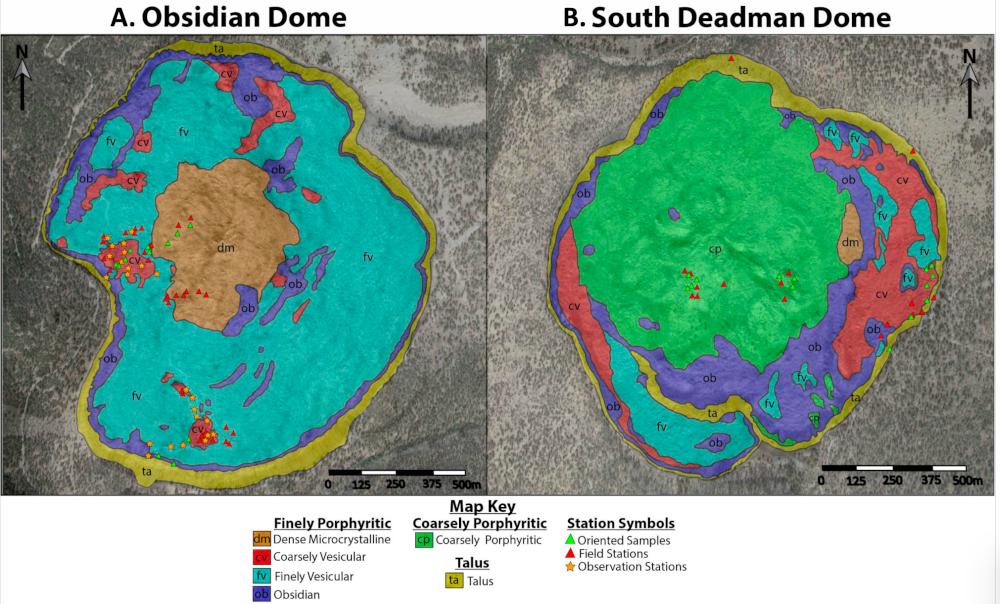
\includegraphics[width=0.95\textwidth]{figs/unitMapping-small.png}
\caption{Textural lithologic distribution maps of lavas for (A) Obsidian dome and (B) South Deadman dome.}
\label{fig:unitMapping}
\end{figure}

\begin{figure}
   \centering
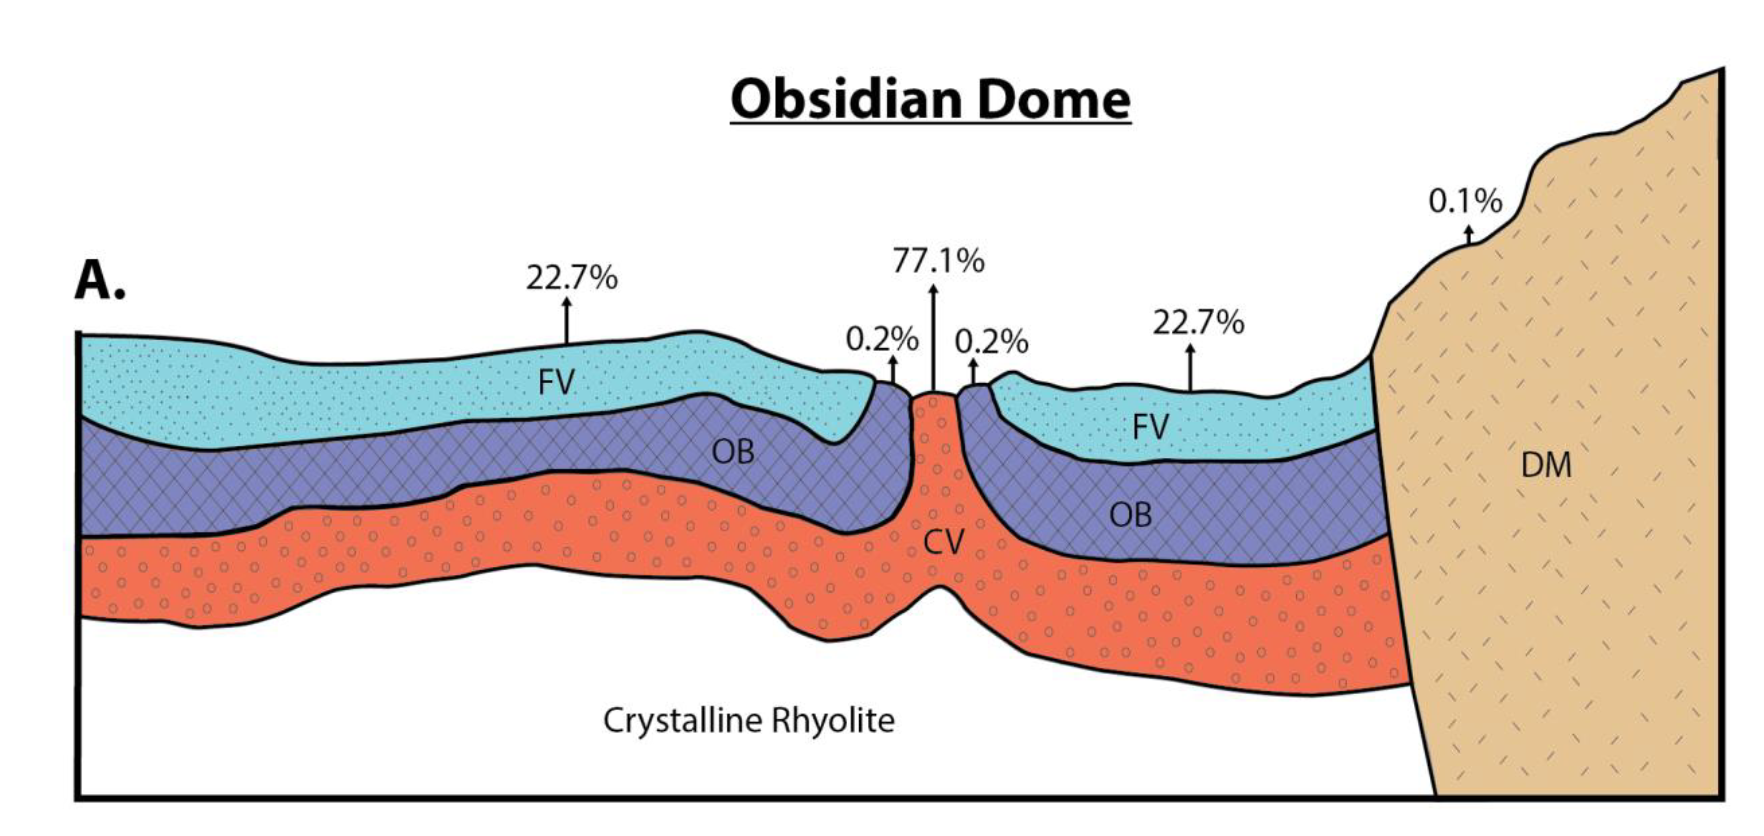
\includegraphics[scale=0.5]{figs/crossSection.png}
\caption{Schematic diagrams depicting total calculated gas flux percentages during the final stages of lava emplacement at Obsidian dome. Total gas flux for each lithologic unit was calculated using the gas flux model of Edmonds et al. (2003), and the gas flux percentages represent the percent gas flux for each lithologic unit relative to the total gas flux calculated for all units, and does not consider additional degassing that occurs through conduit processes, fractures, tuffisite veins, or porous pathways that are too large to measure.}
\label{fig:crossSection}
\end{figure}

\begin{figure}
   \centering
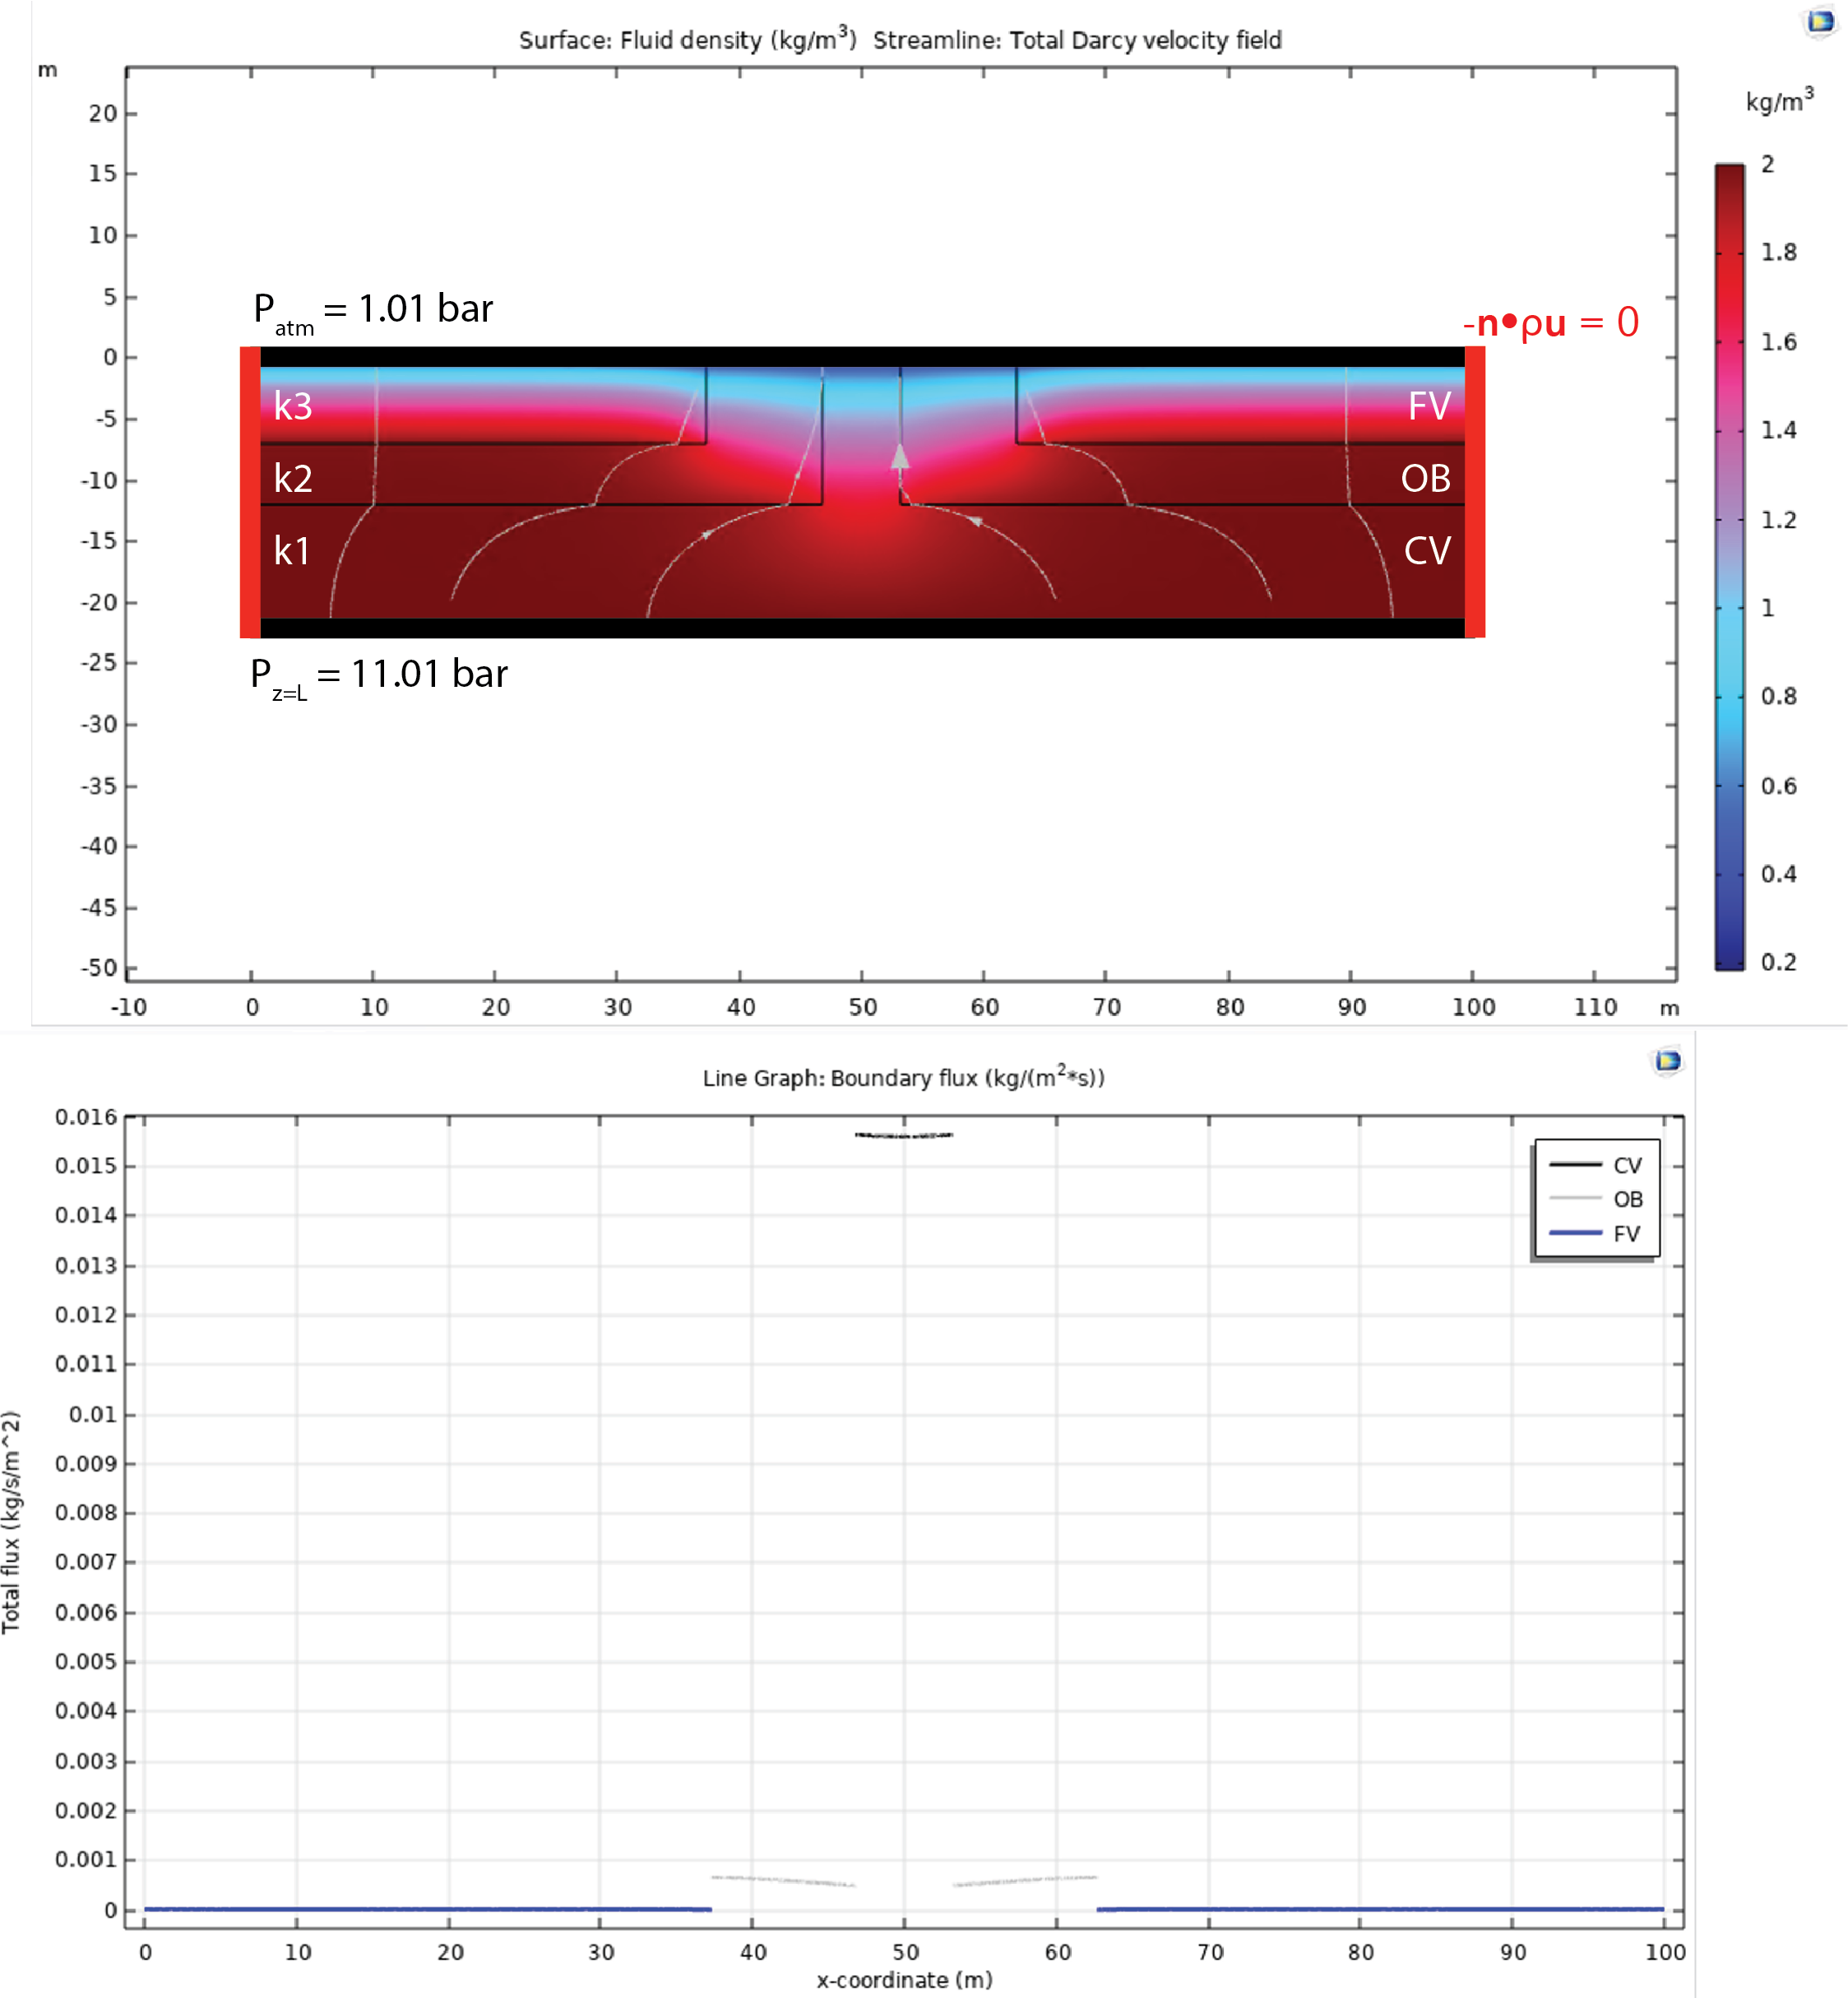
\includegraphics[scale=0.8]{figs/comsolDarcyLaw_units.png}
\caption{Top figure shows gas density in unit layers CV, FV, and OB, with permeabilities k1, k2, and k3, respectively (see Table \ref{tab:UnitPermPoro}). Streamlines indicate the direction of gas flow. Pressure boundary conditions at the base and surface of the units are shown in black, and no flow boundary conditions at the side of the units are shown in red. The bottom figure shows the gas flux at the surface.}
\label{fig:COMSOLresults}
\end{figure}


\begin{table}[h]
\center
      \small
      \begin{tabular}{lllll}
      \hline
      \textbf{Unit} & \textbf{Permeability (m\textsuperscript{2})} & \textbf{Connected porosity (\%)}  & \textbf{Height (m)} & \textbf{Percent of total dome surface area} \\  
      \hline
      CV & 6.87E-12 & 50.0 & 10 & 6.4 \\
      FV & 2.18E-13 & 23.2 &  7 & 74.6 \\
      OB & 4.94E-15 & 3.24 & 5 & 19.0 \\ 
\end{tabular}%}
\caption{Average permeability, porosity, height, and percent of total dome surface area of each textural unit.} 
\label{tab:UnitPermPoro}
\end{table}

\printbibliography

\end{document}
